\documentclass[border=3pt]{standalone}
% Preâmbulo compartilhado pelos diagramas TikZ da aula 5 de IHC (Processos de Design)
\usepackage[T1]{fontenc}
\usepackage[utf8]{inputenc}
\usepackage{lmodern}
\usepackage{amsmath}
\usepackage{xcolor}
\usepackage{tikz}
\usetikzlibrary{arrows.meta,angles,quotes,decorations.pathmorphing,calc,
                positioning,shapes.geometric,shapes.misc,backgrounds,fit,
                math}

% Paleta (mesma dos SVGs originais)
% Paleta da disciplina de IHC: acento roxo (#755099), da capa do livro.
% (o nome "dblue" é mantido para não alterar todos os diagramas)
\definecolor{dblue}{HTML}{755099}
\definecolor{dorange}{HTML}{B3541E}
\definecolor{dgreen}{HTML}{4A7C59}
\definecolor{dred}{HTML}{9C4B4B}
\definecolor{dcream}{HTML}{F4F1EA}
\definecolor{dshade}{HTML}{DDD7C9}

% Função gaussiana (não normalizada por padrão de escala visual)
\pgfmathdeclarefunction{gauss}{3}{%
  \pgfmathparse{1/(#3*sqrt(2*pi))*exp(-((#1-#2)^2)/(2*#3^2))}%
}

% Estilos comuns (prefixo d... para não colidir com chaves internas do pgf)
\tikzset{
  >={Stealth[length=2mm]},
  dguide/.style={gray!55, dashed, line width=0.4pt},
  daxis/.style={gray!60, line width=0.7pt, ->},
  dbody/.style={fill=black!3, draw=black!80, line width=1pt},
  dacc/.style={draw=dblue, line width=1pt},
  dlbl/.style={black!55, font=\small},
  dsub/.style={black!45, font=\footnotesize},
  dstate/.style={circle, draw=black!80, fill=dcream, line width=1pt,
                 minimum size=17mm, font=\large, inner sep=1pt},
  dobs/.style={circle, draw=black!80, fill=dshade, line width=1pt,
               minimum size=14mm, font=\large, inner sep=1pt},
  dbox/.style={rounded corners=2pt, draw=black!80, fill=dcream, line width=1pt,
               align=center, inner sep=6pt},
  dop/.style={circle, draw=black!80, fill=white, line width=1pt,
              minimum size=6mm, inner sep=0pt, font=\small},
  dtrans/.style={->, dblue, line width=1pt},
  dmeas/.style={->, dorange, line width=1pt},
  dcurve/.style={line width=1pt, dblue},
  dcurveb/.style={line width=1.4pt, dorange},
}

\begin{document}
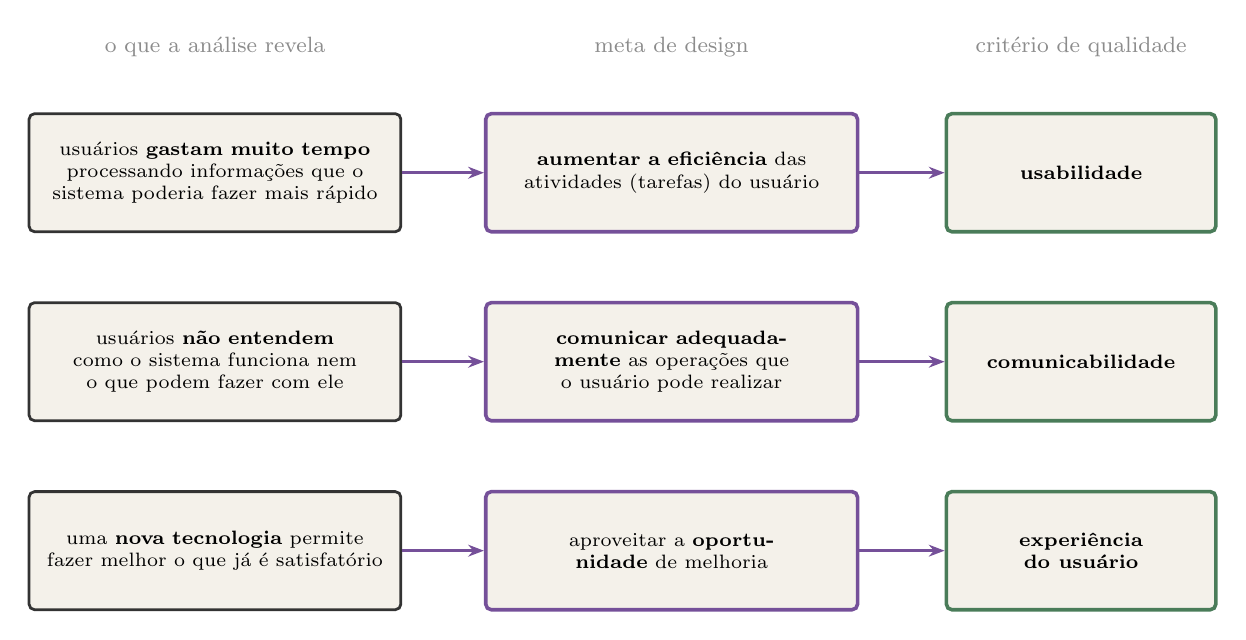
\begin{tikzpicture}[x=1cm,y=1cm,
   obs/.style={dbox, text width=4.3cm, minimum height=1.5cm, font=\scriptsize},
   meta/.style={dbox, draw=dblue, line width=1.3pt, text width=4.3cm, minimum height=1.5cm, font=\scriptsize},
   crit/.style={dbox, draw=dgreen, line width=1.3pt, text width=3.0cm, minimum height=1.5cm, font=\scriptsize\bfseries}]

  \node[font=\scriptsize\bfseries, dsub] at (2.2,3.6) {o que a análise revela};
  \node[font=\scriptsize\bfseries, dsub] at (8.0,3.6) {meta de design};
  \node[font=\scriptsize\bfseries, dsub] at (13.2,3.6) {critério de qualidade};

  \node[obs] (o1) at (2.2,2.0) {usuários \textbf{gastam muito tempo} processando informações que o sistema poderia fazer mais rápido};
  \node[meta] (m1) at (8.0,2.0) {\textbf{aumentar a eficiência} das atividades (tarefas) do usuário};
  \node[crit] (c1) at (13.2,2.0) {usabilidade};
  \draw[dtrans] (o1) -- (m1); \draw[dtrans] (m1) -- (c1);

  \node[obs] (o2) at (2.2,-0.4) {usuários \textbf{não entendem} como o sistema funciona nem o que podem fazer com ele};
  \node[meta] (m2) at (8.0,-0.4) {\textbf{comunicar adequadamente} as operações que o usuário pode realizar};
  \node[crit] (c2) at (13.2,-0.4) {comunicabilidade};
  \draw[dtrans] (o2) -- (m2); \draw[dtrans] (m2) -- (c2);

  \node[obs] (o3) at (2.2,-2.8) {uma \textbf{nova tecnologia} permite fazer melhor o que já é satisfatório};
  \node[meta] (m3) at (8.0,-2.8) {aproveitar a \textbf{oportunidade} de melhoria};
  \node[crit] (c3) at (13.2,-2.8) {experiência do usuário};
  \draw[dtrans] (o3) -- (m3); \draw[dtrans] (m3) -- (c3);

\end{tikzpicture}
\end{document}
